\documentclass[]{article}
\usepackage[hidelinks]{hyperref}
\usepackage{graphicx}
\usepackage[inline]{enumitem}
\usepackage{listings}
\usepackage{subcaption}
%opening



\begin{document}

\begin{flushleft}

\centering { \large \bf Comparative Evaluation of Spark and Flink Stream Processing}
\vspace{4pt}

\centering
 MA-INF 4306 - Data Science and Big Data \\
 Lab Report\\
 
   Winter Semester 2016.17\\

		 University of Bonn\\


\vspace{6pt}
\centering
 Ehab Qadah\\
 Supervisor: PD Dr. Michael Mock.
 \vspace{4pt}
 
 \today
\end{flushleft}


\begin{abstract}

\end{abstract}
Recent years have witnessed advances in the  development of Big Data frameworks like Apache Spark and Apache Flink. For instance, both frameworks support real-time data 
stream processing. The question of which platform is superior to the other still open. 
In this report, we provide a performance comparison of streaming data processing in Apache Spark and Apache Flink by measuring different performance metrics (latency and throughput). Furthermore, we cover some key aspects of streaming data applications and how they are handled in the two frameworks. The experiment is done using multiple streaming workloads over real-world datasets. Results show that Flink outperform Spark streaming in term of latency. While Spark Streaming gives higher throughput rates than Flink. 
\section{Introduction}

\par In recent years, Big Data is considered as one of the most appealing topics in Information Technology, it has gained increasing attention of professionals in industry and academia. This attention is a result of the fact that the amount of data we generate is increasing exponentially \cite{idc}.  Different sources such as  social media platforms, mobile phones, Internet of things (IoT), financial transactions, etc.  create large volumes of data.  Moreover, many Big Data frameworks have been recently developed such as Apache Spark and Apache Flink that provide efficient data processing functionalities.
 \par Big Data is a term that does not only describe large datasets (volume), but also the data that arrives in high rate (velocity), and it comes in a mix of different data format (variety) (i.e., 3Vs of Big Data (Volume, Velocity, Variety)) \cite{svs}.

\par The processing models of Big Data are Batch processing and Stream processing. Batch processing involves handling  large, finite volumes of data (e.g., processing of historical transaction records), and is more concerned with throughput. While Stream processing  is a method to manage fast and continuously incoming data (real-time), as it arrives to the system (e.g., credit card fraud detection and network monitoring applications). Stream processing systems usually  provide low latency processing. Both processing models are capable of operating with structured or semi-structured data (i.e., variety).

\par There exist some publications that compare Apache Spark and Apache Flink
 such as the Yahoo Streaming Benchmark \cite{yahoo}. But we believe that we still need to carry our evaluation for two reasons: \begin{enumerate*}[label=(\roman*)]
\item both frameworks are continuously improving in short time 
\item we aim to study the performance of some complex operations such as \texttt{groupByKey} \& \texttt{keyBy} in Apache Spark and Apache Flink, respectively.
\end{enumerate*}

 

\par The purpose of this report is to provide a comparative experimental evaluation of throughput and latency of stream processing in Apache Spark and Apache Flink. In order to simulate real-world use cases, we use datasets of airplane trajectories provided by the  Datacron project\footnote{\url{http://www.datacron-project.eu/}} to develop multiple streaming data processing workloads. Beside the performance comparison of the stream processing of the two frameworks, we try to cover general aspects of stream processing tasks (see Section 3) and how they can be solved in each platform. Informally,  this work aims to help the developers to determine which platform to use for different use cases. 


\par The remainder of this report is organized as follows.
In Section 2, we present the main characteristics, programming APIs, and main data abstraction of Apache Spark and Apache Flink. Section 3  presents the general aspects of stream processing tasks and the implementation of experimental workloads. Section 4
compares the performance results of the different workloads. And finally, Section 5 gives the overall conclusion.

\section{Technical Background}
 In this section, we present the architecture, key characteristics, programming APIs  of Apache Spark and Apache Flink. Moreover, a brief overview of the Apache Kafka platform is  provided.

\subsection{Apache Spark}

\par Apache Spark is an open source project that provides a general framework for large-scale data processing \cite{spark}. It offers programming APIs in Java, Scala, Python and R. Its stack includes a set of built-in modules including Spark SQL, MLlib for machine learning, GraphX for graph processing, and Spark Streaming to process real-time data streams. It can access different data sources including Hadoop Distributed File System (HDFS), Apache Cassandra database, Apache HBase database etc.

\par The main data abstraction of Spark core is the Resilient Distributed Datasets (RDDs), which is in-memory collection of elements partitioned across cluster of computers that can be processed in parallel \cite{rdd}. RDDs support two categories of operations: transformations that drive new RDDs from the operated ones (e.g., \texttt{map}, \texttt{filter} and \texttt{groupByKey}), and actions which return a certain value (e.g., \texttt{count} and \texttt{collect}). Additionally, Discretized Stream (DStream) is the data abstraction in Spark Streaming, which is a series of RDDs that represent an input stream of data \cite{spark_streaming}. In other words, the Spark Streaming is a batch-based processing model, which processes the continuous stream of data by dividing it into micro-batches that are  processed by the Spark engine. Figure 1 illustrates the general process flow of Spark Streaming. 


\begin{figure}[h]
 
  \centering
    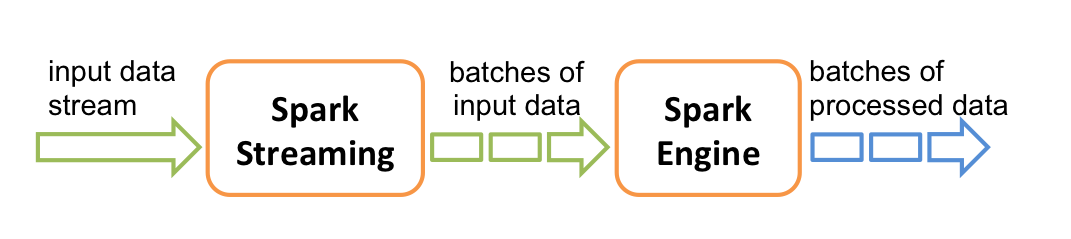
\includegraphics[width=.9\textwidth, height=.3\textheight]{streaming-flow.png}
     \caption{ Process flow of Spark Streaming \cite{spark_streaming}.}
\end{figure} 

\subsection{Apache Flink}

\par Apache Flink is an open source project that provides a large-scale, distributed stream processing platform \cite{flink}. Flink treats the batch processing as special case of streaming applications (i.e., finite stream).
It offers programming APIs in Java and Scala. Its software stack includes the core DataStream and DataSet APIs with additional libraries such as Complex event processing for Flink (FlinkCEP), Machine Learning for Flink (FlinkML)  and Flink Graph API (Gelly).

\par The main data abstraction of Flink are DataStream and DataSet that represent read-only collection of data elements. The list of elements is bounded (i.e., finite) in DataSet, while it is unbounded (i.e., infinite) in case of DataStream.

\par The Flink's core is a distributed streaming dataflow engine,  with each Flink program is represented by a dataflow graph (i.e., directed acyclic graph - DAG) that executed by the Flink's engine \cite{flink_paper}. The data flow graphs are composed of stateful, parallel operations and intermediate data stream partitions. Figure 2 shows a data flow graph of a Flink program.


\begin{figure}[h]
 
  \centering
    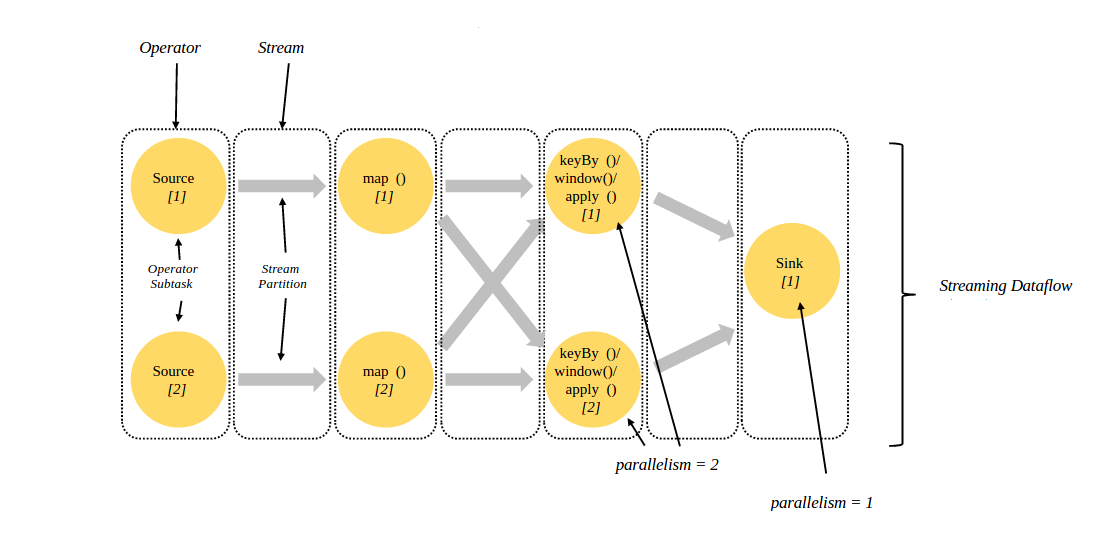
\includegraphics[width=\textwidth, height=.5\textheight]{flink_engine.png}
     \caption{ An example of data flow graph in Flink \cite{flink}.}
\end{figure} 
\newpage
\subsection{Apache Kafka}
\par Apache Kafka is scalable, fault-tolerant and distributed streaming framework \cite{kafka}. It allows to publish and subscribe to data streams.
Kafka manages the stream records in different categories (i.e., topics) that are partitioned and distributed over the servers of the Kafka cluster. It allows the data producers to publish a stream of records to one or more  Kafka topic. Additionally, consumer applications can subscribe to one or more topic to read data streams. The consumers within a group use the  same group name, which allows Kafka to distribute and balance the stream partitions among the  members of a certain group for the sake of scalability. Figure 3 shows how 4 partitions of a stream are distributed between two groups of consumers based on the number of members. 
Apache Kafka has been widely  adopted, for example, 
Apache Spark and Apache Flink can ingest Kafka streams. 

\begin{figure}[h]
 
  \centering
    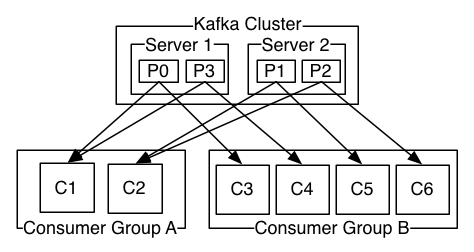
\includegraphics[width=\textwidth, height=.4\textheight]{kafka_groups.png}
     \caption{ Distribution of a stream partitions for consumer groups in Kafka \cite{kafka}.}
\end{figure} 

\newpage
\section{Experiment Setup and Implementation}
This section describes the data stream setup, the design of evaluation streaming workloads and the  implementation details of the proposed solution of Apache Spark and Apache Flink.

\subsection{Data Stream Setup}
The evaluation streaming workloads read an input data stream from Kafka. In order to simulate real-world use case we use datasets of Automatic Dependent Surveillance – Broadcast (ADS-B) messages that represent the aircraft's position over time. The message line comprises 22 fields of data such as aircraft ID, date message generated, longitude, latitude and altitude.  And  these datasets contain around \texttt{26 millions} messages.  
\par In our experiment a data stream producer component reads the ADS-B message datasets, then publishes them to the Kafka cluster to be consumed by the workloads in Apache Spark and Apache Flink. Figure 4 illustrates the data producer and the Kafka cluster setup in all experiments.
The data stream is divided into four portions over two server. The data producer publishes the stream records randomly to a Kafka partition and all ADS-B messages are published to the same topic (\texttt{datacorn}). Moreover, the data producer attaches the time of publishing to the ADS-B message line before publishing it to the Kafka topic.

\begin{figure}[h]
 
  \centering
    \includegraphics[width=.9\textwidth, height=.3\textheight]{kafka.png}
     \caption{The setuop of the Data Stream Producer \& Kafka Cluster.}
\end{figure} 

\newpage
\subsection{Evaluation Streaming Workloads}
In our experimental evaluation, we developed two real-time stream processing workloads that read a ADS-B messages stream from Kafka in order to perform basic trajectories analysis methods. The workloads are designed to cover general key aspects of real-time stream processing tasks and evaluate the corresponding solutions in Spark and Flink. The following are the aspects of streaming data processing were covered by our workloads's design: 

\begin{itemize}
\item Handling parallel input streams (e.g., Kafka Stream).
\item How to aggregate the state of input stream.
\item Manage the order of stream records.
\item How to provide and update global data model in a stream processing task.
\item Evaluate the performance by measuring the latency and throughput.
\end{itemize}
We give the description of workloads, the relation with these aspects and  the implementation details of Spark's and Flink's solutions in Sections 3.2.1 \& 3.2.1. Afterward, In Section 4 we discuss the performance evaluation and analysis of stream processing workloads in the two frameworks. 
\par The two streaming workloads and the data stream producers are implemented in Java and the source code is available in a repository on Github\footnote{\url{https://github.com/ehabqadah/Spark_vs_Flink}}. 

\subsubsection{Statistics Computation per Trajectory}
In the first stream processing workload, we construct a stream of trajectories by considering  the position messages (i.e., ADS-B messages) that belong to the same aircraft as trajectory. Moreover, we continuously compute and aggregate statistics for each new position in a trajectory . As example of computed statistics quantities speed mean, mean of location coordinates, min and max altitude, etc. In this workload, we cover the parallel receiving of input data stream, statefull aggregation over the input data stream, and preserving the correct order of the stream's records.
The implementation details of this workload in Spark and Flink are presented in the following: 
\begin{itemize}
\item {\bf{Implementation in Spark }}

\par The implementation of trajectory statistics computation in Spark Streaming, first, it reads the Kafka stream using \texttt{KafkaUtils.createDirectStream} that creates \texttt{DStream} that represents the stream of position messages, in order to scale up and have parallel Kafka stream receivers, a multiple instances of \texttt{DStream} must be created and combined together using the \texttt{union} operation. The output stream of the \texttt{union} is further processed using \texttt{mapToPair}, to map each position message to tuple of aircraft ID and position message. Then, the irrelevant tuples are filtered based on the position message type using  a \texttt{filter} transformation. Afterward, the tuples that share the same aircraft ID are groped together to construct the stream of trajectories (tuples of Id and list of positions), by applying the \texttt{groupByKey} operation. Since the processing  model of Spark Streaming is micro-batch based and stateless, \texttt{updateStateByKey} operation must be used to maintain the state of the trajectories stream. In the context of this workload, the state is the aggregated statistics of trajectory, so the statistics computation is preformed within the custom \texttt{updateStateByKey} function that is continuously applied for every batch.
 The state update function uses the last position of trajectory from previous batch to aggregate and compute statistics quantities to each trajectory's position in the new data batch, and the new positions list is kept as the new state for the trajectory. Inside the state update function, the new positions must be sorted to preserve the correct order, since the tuples after \texttt{groupByKey} operation are shuffled across the cluster's  nodes and sent to the state update function.

\item {\bf{Implementation in Flink }}


The details of Flink's implementation of statistics computation workload as follows. First, a \texttt{FlinkKafkaConsumer} is used to  construct a \texttt{DataStream} instance that represent the Kafka stream of aircrafts positions, it implicitly runs multiple parallel Kafka stream consumers, which makes the Kafka partitions balanced between the instances. Second, the stream records (i.e., ADS-B messages) are parsed and transformed to tuples of ID and position message using a configured \texttt{map} transformation. Third, a \texttt{filter} function is used to filter irrelevant tuples based on the message type. Fourth, the resulted tuples after the filtration transformation are grouped based on the tuple's ID using \texttt{keyBy} operator that constructs the \texttt{KeyedStream} of trajectories. Finally, 
a \texttt{reduce} transformation on the  \texttt{KeyedStream} is used to calculate the statistics for each new coming trajectory's position, by utilizing the aggregated statistics of previous position, while old position is discarded and the new position with attached computed statistics is used to aggregate the statistics of a certain trajectory.

\end{itemize}

\par In summary, Flink  handles  the parallel consumers of Kafka stream implicitly, while a multiple \texttt{DStream} must be created in Spark Streaming and union them to have parallel Kafka receivers. The Flink's streaming processing is stateful that means there is no need to manage the stream state as the case in Spark streaming. A sort action is required in Spark Streaming to preserve the correct  order of the position messages inside the state update function.

\subsubsection{Air Sector Change Detection}

The goal of sector change detection workload is to detect the  entering or leaving of an aircraft from one air sector to another one, by processing the real-time stream of aircraft positions. Given the fact that a dataset of sectors (i.e., polygons) is available as a reference to assign the corresponding sector for certain aircraft's position. In this workload, we test the aspect of providing a global data model (sectors dataset) in stream processing workload. Moreover, the preserving of the stream's records order and consuming of parallel Kafka streams  are covered.
 
 The implementation details of this workload in Spark and Flink are presented in the following: 
 
 \begin{itemize}
 \item {\bf{Implementation in Spark }}
 
 We implemented the sector change detection workload in Spark Streaming by constructing the stream of trajectories and assigning a sector for each position of a trajectory. A change between the assigned sectors of two consecutive aircraft's positions is marked  as a transition of sector for a certain trajectory. \par First, multiple instances of \texttt{DStream} are created using \texttt{KafkaUtils.create} \texttt{DirectStream}  are combined using \texttt{union} to read in  parallel from Kafka. Second, the records (i.e., ADS-B messages) of the resulting stream are parsed and mapped to tuples of (aircraft ID, position message) using \texttt{mapToPair} transformation. Third, the unrelated  tuples are filtered based on the message type using a \texttt{filter} operation. Fourth, the stream of trajectories is constructed by combining all tuples with the same ID using the \texttt{groupByKey} function. Then, to manage and aggregate the state of trajectories stream between the mini-batches a configured \texttt{updateStateByKey} function is applied. The state update function assigns the corresponding sector for each new position, the old positions of a certain trajectory from the previous batch are discarded, but only the last position of the old batch is kept to be used alongside with the new positions. In addition to that the new positions are sorted by th streaming time to maintain the correct order.
 \par The sector data set is provided using the built-in \texttt{Broadcast} feature that distributes a shared value for  all cluster nodes in an efficient matter. Finally, the detection of a sector change is done by an extra filtering transformation using a \texttt{filter} operator, which checks the sectors of consecutive positions in a trajectory to find the ones with a change in the sector assignment.

 
  
 \item {\bf{Implementation in Flink }}
 
 The Flink's implementation of sector change detection workload uses the \texttt{FlinkKafkaConsumer09} that reads the position messages (i.e., ADS-B) stream from Kafka, which is used to construct a \texttt{DataStream} instance. The \texttt{DataStream}'s records are mapped to tuples of (aircraft ID and aircraft's position) by a configured \texttt{map} transformation. Irrelevant tuples are filtered based on the message type using a \texttt{filter} operation. Afterward, the tuples that shares a common IDs are grouped together by the \texttt{keyBy} operator. Since the Flink streaming processes the stream records as it come, a defined \texttt{reduce} operator assign corresponding sector of position on new tuple, while the old tuple with same ID is used to retrieve the previous sector to attach it to the new tuple, while the old tuple is discarded. Finally, the tuples (i.e., tuple of (aircraft ID, position message)) with different previous and current sector are filtered using defined \texttt{filter} transformation.

 \end{itemize}
 
 
 \par To sum up, the same differences between Flink and Spark Streaming regarding the state management and parallel  consumers of Kafka stream as was discussed in Section 3.2.1. Another key difference between them, is how  to provide the global data model (e.g., sectors) in a streaming workload. Spark Streaming offers the \texttt{Broadcast} feature to handle this issue in efficient way, while the global data model is manually provided  to the stream operations in Flink.
\section{Performance Results}

\par This section presents the results of performance evaluation in Spark (2.0.2) and Flink (1.1.3) for the streaming workloads that were described in Section 3.2. Specifically, we provide  the measurements of latency and throughput of the benchmarking workloads execution in Spark Streaming and Flink. We carried the experiment by setting up the Kafka stream as described in Section 3.1 on a local machine\footnote{ The experiments have been carried  on single machine with Ubuntu 16.04 LTS os, Intel® Core™ i5-6200U CPU @ 2.30GHz × 4  processor, and 16 GB of memory.} and execute the different workloads on the same machine (i.e., local mode) to obtain the performance results.  

\par We consider the time delay between the streaming time of a record in Kafka and  the time when the record is processed by a workload as the platform's processing latency (measured in milliseconds). And the number of processed stream's records (aircrafts position messages) per second within each streaming workload is the throughput measure. Since the Spark Streaming is micro-batch based,  we examine the effect of different batch intervals
of the Spark Streaming on the performance measurements.


\subsection{Latency Results}

Figure 5 shows the results of the latency measurements of the streaming workloads in Spark and Flink. The presented values present the average value of multiple trails and measurements. Measurements for different batch durations are given in Spark Streaming, we noticed that making the batch time too small does not give better latency results. Results show that Flink outperform Spark streaming in term of processing latency in the two evaluation workloads.

\begin{figure}[h]
\centering
\begin{subfigure}{.7\textwidth}
  \centering
  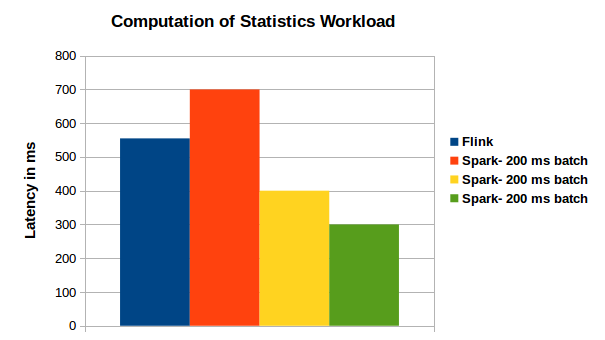
\includegraphics[width=\linewidth]{latency1.png}
  \caption{Latency of Statistics Computation}

\end{subfigure}%
\vskip\baselineskip
\centering
\begin{subfigure}{.7\textwidth}
  \centering
  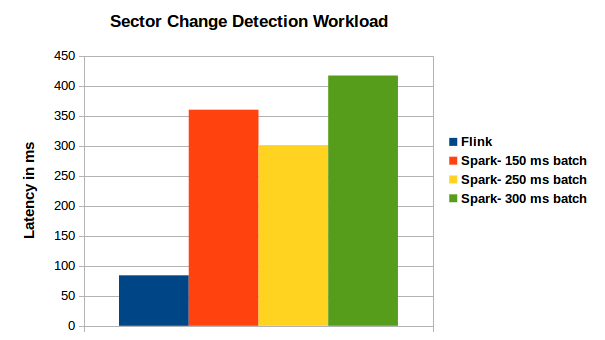
\includegraphics[width=\linewidth]{latency2.png}
\caption{Latency of Sector Change Detection }

\end{subfigure}
\caption{Latency Measurements}
\label{fig:fig}
\end{figure}
\newpage
\subsection{Throughput Results}

The  measurements of throughput for the two streaming workloads are given in Figure 6. The presented values reflect the average of throughput (message/minute) 
 in Spark streaming and Flink for multiple executions. Also for Spark streaming we tested different 
 batch times. Results show that Spark Streaming has higher throughput than Flink, also  increasing the batch duration of Spark Streaming gives better throughput.

\begin{figure}[h]
\centering
\begin{subfigure}{.7\textwidth}
  \centering
  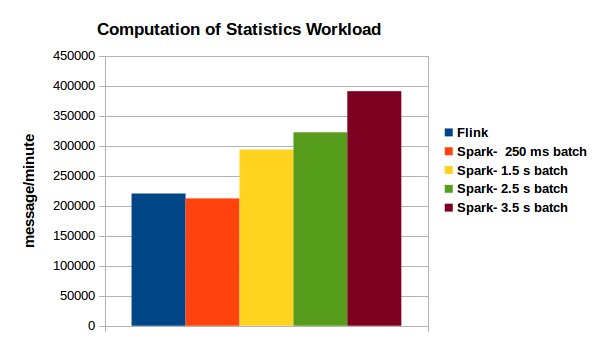
\includegraphics[width=\linewidth]{throughput1.png}
  \caption{Statistics Computation}

\end{subfigure}%

\vskip\baselineskip
\centering
\begin{subfigure}{.7\textwidth,}
  \centering
  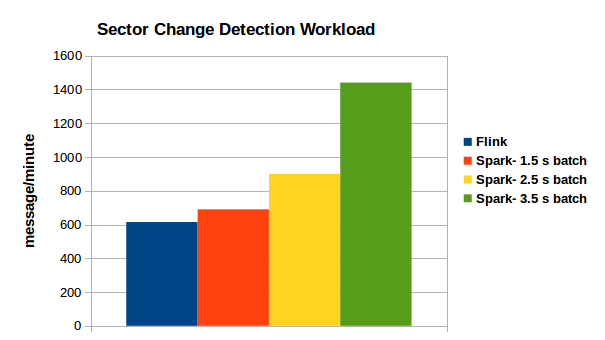
\includegraphics[width=\linewidth]{throughput2.png}
\caption{Sector Change Detection }

\end{subfigure}
\caption{Throughput Measurements}
\label{fig:fig}
\end{figure}


\section{Conclusion}

In this report, we present an experimental evaluation of the stream processing performance and capabilities of Apache Spark and Apache Flink. We carried our experiment over aircraft positions datasets provided by the Datacorn project, we developed two streaming workloads to cover general aspects of real-time stream processing tasks. Additionally, and we measured the latency and throughput of those workloads solution of Spark and Flink. Results show that Flink outperforms Spark Streaming in term of processing latency. In contrast, Spark Streaming has showed better throughput rates than Flink. 
\par To sum up, Flink's processing model is well-suited to the stream processing tasks that require low latency, also there is no need to manage the Stream's state and the batch interval in contrast to Spark streaming. Moreover, Flink operates over the individual record of the data stream, while Spark Streaming  processes the input data stream as micro-batches. Thus we can state that  Flink is a true stream processing framework. A side remark, we have  noticed that finding online resources related to Spark is easier than to Flink.

In future work, we plan to carry our experiments over cluster of computers not just only on single computer. In addition, we will cover more aspects of real-time data stream processing and developing more evaluation workloads. 


\begin{thebibliography}{[MT1]}
%
\bibitem[1]{idc} 
Gantz, John, and David Reinsel. "The digital universe in 2020: Big data, bigger digital shadows, and biggest growth in the far east." IDC iView: IDC Analyze the future 2007.2012 (2012): 1-16.

\bibitem[2]{svs} 
Laney, D 2001 3D Data Management: Controlling Data Volume, Velocity, and Variety. META Group.

\bibitem[3]{yahoo} 
Chintapalli, Sanket, et al. "Benchmarking streaming computation engines: Storm, Flink and Spark streaming." Parallel and Distributed Processing Symposium Workshops, 2016 IEEE International. IEEE, 2016.

\bibitem[4]{spark} 
Apache Spark. Available: https://spark.apache.org/ [Accessed February 2017].

\bibitem[5]{rdd}
Zaharia, Matei, et al. "Resilient distributed datasets: A fault-tolerant abstraction for in-memory cluster computing." Proceedings of the 9th USENIX conference on Networked Systems Design and Implementation. USENIX Association, 2012.

\bibitem[6]{spark_streaming}
Spark Streaming. Available: http://spark.apache.org/docs/latest/streaming-programming-guide.html [Accessed March 2017].

\bibitem[7]{flink} 
Apache Flink. Available: https://flink.apache.org/ [Accessed February 2017].

\bibitem[8]{flink_paper} 
Carbone, P., Katsifodimos, A., Ewen, S., Markl, V., Haridi, S. et al. (2015)
Apache flink: Stream and batch processing in a single engine.
Bulletin of the IEEE Computer Society Technical Committee on Data Engineering, 36(4).

\bibitem[9]{kafka} 
Apache Kafka. Available: https://kafka.apache.org/intro.html [Accessed February 2017].

%
\end{thebibliography}
\end{document}
